%! Author = mboehme
%! Date = 01.03.2023

\newpage
\section{Ergebnis}\label{sec:ergebnis}
Abgleich der Ergebnisse mit den Soll-Anforderungen.
\subsection{Visuelle Darstellung}\label{subsec:visuelle-darstellung}
%include two images
%\par\vspace{1cm}
%\begin{figure}[h]
%    \centering
%    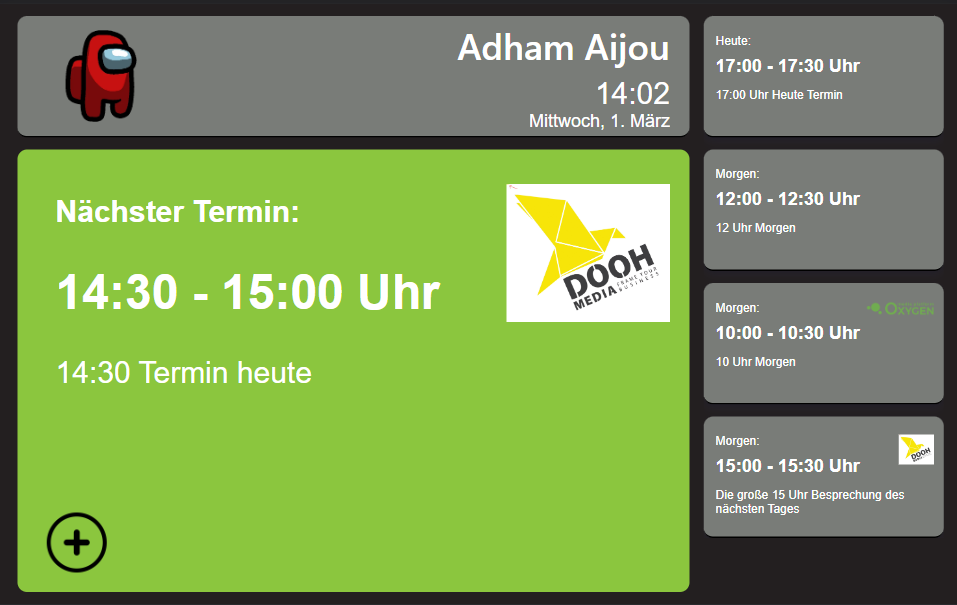
\includegraphics[width=0.8\textwidth]{Bilder/Ergebnis}
%    \caption{Ergebnis mit nächstem anstehenden Termin}
%    \label{fig:Ergebnis mit nächstem anstehenden Termin}
%\par\vspace{1cm}
%\end{figure}
%\justifying
%\par\vspace{1cm}
\begin{figure}[h]
    \centering
    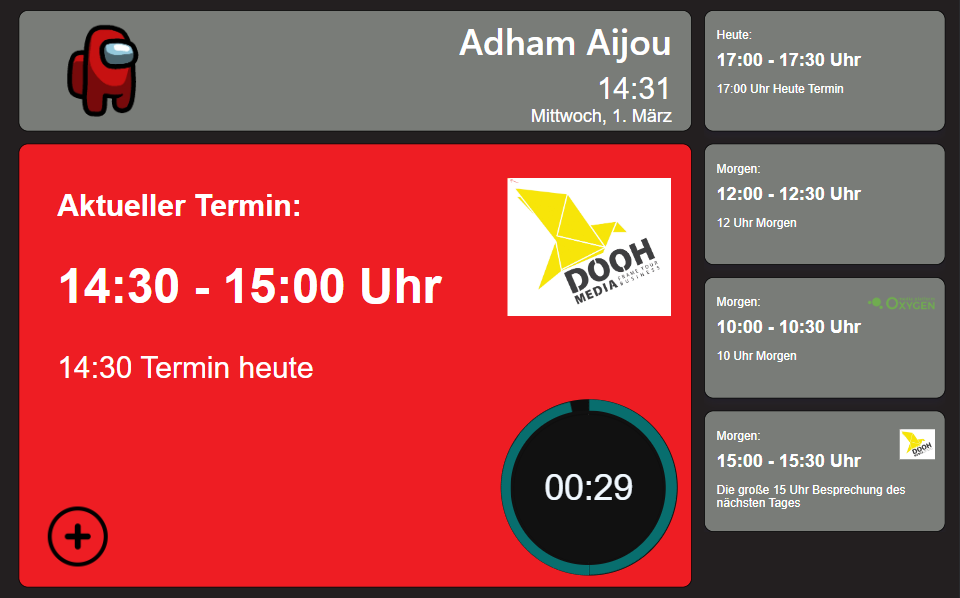
\includegraphics[width=0.8\textwidth]{Bilder/Ergebnis_LaufenderTermin}
    \caption{Ergebnis mit laufendem Termin}
    \label{fig:Ergebnis mit laufendem Termin}
\par\vspace{1cm}
\end{figure}
\justifying
\newline
Oben links im Bild, ist das Logo des Gastgebers des nächsten, beziehungsweise jetzigen, Termins zu sehen.
In diesem Fall ist dies das Logo der DOOH media GmbH\@.
Solch ein Logo kann dargestellt werden, indem beim Erstellen des Termins, außerhalb des Tablets, bei Outlook beispielsweise, ein Bild an den Termin angehangen wird, welches im Dateinamen \("\)Termin\_Logo\("\) enthält.
\newline
Die anderen Logos sind alle Logos vom Gast des Termins.
Sie werden angezeigt, indem der Firmenname im Textkörper des Termins vorkommt.
Um diese Logos initial den Firmennamen zuzuordnen, muss ein spezieller Termin erstellt wird, der nur für die Logos gedacht ist und eine einzigarte ID, sowie einen Befehl enthält, die dann das Bild, inklusive Firmennamen, in einer lokalen Datenbank abspeichert.
Diese Logos können hinzugefügt, gelöscht oder aktualisiert werden.
\newline
Die Uhrzeit wird immer in der Zeitzone des Tablets angezeigt.
\newline
\newline
%Das gehört in sollzustand.
Hier sieht man das Menü, in welchem ein Termin gebucht werden kann, welches durch das Drücken des Plus-Symbols aufgerufen wird:
\begin{figure}[h]
\par\vspace{1cm}
    \centering
    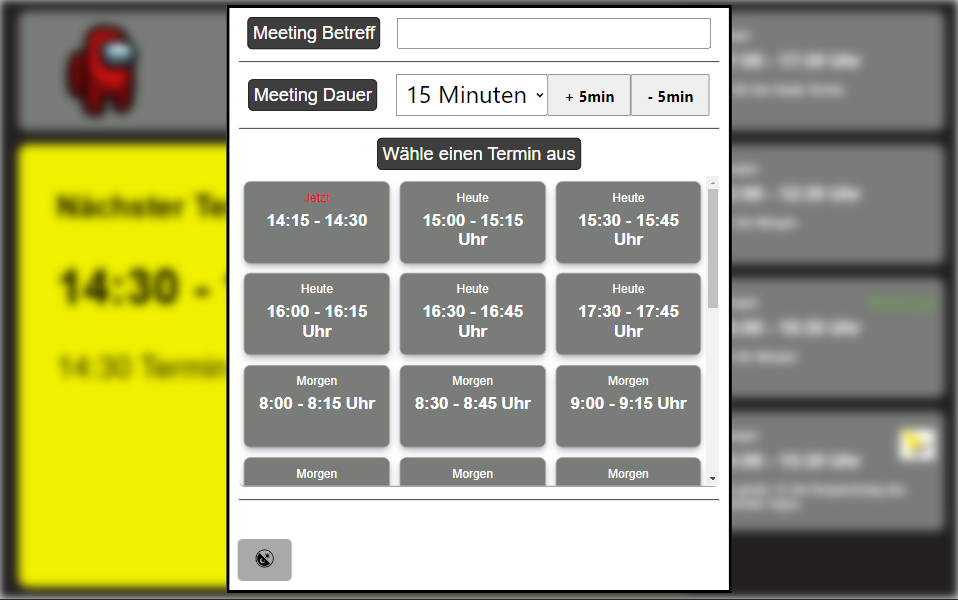
\includegraphics[width=0.8\textwidth]{Bilder/Ergebnis_TerminErstellen_Menue}
    \caption{Terminbuchungsmenü}
    \label{fig:Menue}
\par\vspace{1cm}
\end{figure}
\justifying
\pagebreak

Die \("\)Jetzt\("\) Option wird im Terminbuchungsmenü nicht angezeigt, weil bereits ein Termin stattfindet.
Falls ein kein Termin stattfindet, wird eine \("\)Jetzt\("\) Option angezeigt.
Wenn das Ende des \("\)Jetzt\("\) Termins innerhalb von 15 Minuten vom nächsten anstehenden Termin beginnt, wird der \("\)Jetzt\("\) Termin rot markiert, sodass der Nutzer weiß, dass er den Termin nicht buchen kann, weil er zu lange dauert.
Diese Option ist dann auch deaktiviert.
So wird dem Nutzer übermittelt, dass die Option generell schon verfügbar ist, aber nur falls die Dauer verkürzt wird.
Es werden alle möglichen Termine, innerhalb der Arbeitszeiten, für den Jetzigen und nächsten Tag angezeigt.
Falls z.B. der nächste Tag ein Feiertag ist, werden für den nächsten Tag keine Termine angezeigt.
Auf die anderen Optionen, wie z.B. Pufferzeiten, hat ein Anwender hier wenig Einfluss, da sie von den Einstellungen des Kalenders, des jeweiligen Nutzers, abhängen und es somit in der Verantwortung des Administrators liegt, diese zu ändern.
\newline
\newline
%Hier die normale Ansicht nochmal, im hellen Design:
%\par\vspace{1cm}
%\begin{figure}[h]
%    \centering
%    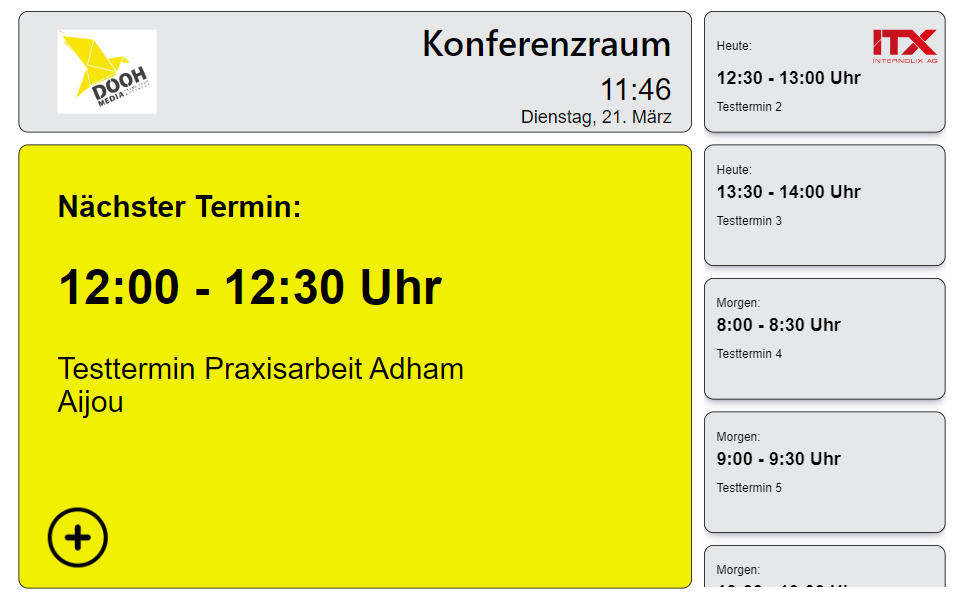
\includegraphics[width=0.8\textwidth]{Bilder/Ergebnis_lightMode}
%    \caption{Ergebnis im hellen Design}
%    \label{fig:Ergebnis im hellen Design}
%\par\vspace{1cm}
%\end{figure}
%\justifying
%\newline
%\newline
%\pagebreak
%Eigenes Kapitel

\subsection{Ausblick}\label{subsec:ausblick}
\subsubsection{kurzfristig}\label{subsubsec:kurzfristig}
Die Software wird vom Kunden eingesetzt.
Da dies ein Pilotprojekt ist, wird die Software nur von einem Kunden genutzt.
Dafür wurden acht Tablets angeschafft, die an den Räumen des Kunden installiert werden.

\subsubsection{mittelfristig}\label{subsubsec:mittelfristig}
Der Kunde wird die Anwendung erstmal benutzen müssen.
Rückmeldungen werden gesammelt und kritische Fehler werden behoben.
Trotz ausgiebigen Tests, kann es immer noch zu Fehlern kommen, die erst im Einsatz auffallen.
\subsubsection{langfristig}\label{subsubsec:langfristig}
Die Schnittstelle wurde nicht vollständig genutzt, da die Anwendung nicht alle Funktionen benötigt, aber sie bietet für die Zukunft viele Erweiterungsmöglichkeiten.
Mit der gesammelten Erfahrung und den gewonnenen Erkenntnissen kann die Anwendung in Zukunft erweitert werden.
Zudem ist die API neu und wird ständig weiterentwickelt~\cite{microsoft-graph-api-version}.
Insbesondere mit den jüngsten Entwicklungen von künstlichen Intelligenzen, wie z.B. der Spracherkennung, könnte die Anwendung erweitert werden.

\subsection{Fazit}\label{subsec:fazit}
%Für die Anwendung wurde die Schnittstelle genutzt, um Termine zu erstellen, zu löschen und zu aktualisieren.
%Außerdem wurde die Schnittstelle genutzt, um die Logos der anderen Termine zu erhalten.
%
%Für den Anwendungsfall des Kunden ist die API ausreichend, da die Anwendung nur Termine erstellen, löschen und aktualisieren können muss.
%Alles Weitere wird von der Webapplikation abgedeckt.
%Der einzige Nachteil ist, dass Azure AD, die Authentifizierung, für Ressourcenkonten nicht unterstützt, die beispielsweise, in Teams, genutzt werden.
%Daher muss der Anwender sich mit einem Microsoft-Konto anmelden, welcher die Ressource repräsentieren soll, aber nicht ein Ressourcenkonto ist.
%Dies kann zu Verwirrung führen, da die Terminologie impliziert, man könne sich mit einem Ressourcenkonto anmelden.
%\newline
%\newline
%Die API war die richtige Wahl für diesen Kundenauftrag.
%Ressourcen- und Terminplanung wurde mit der Anwendung vereinfacht.
%Ein Anwender braucht nur noch drei Klicks, um einen Termin zu erstellen und muss nicht mehr zwischen verschiedenen Kalendern hin und her wechseln.
%%Aua, Fixen, umformen
%Zudem benötigt ein Anwender lediglich einen Blick, um zu sehen, wann die Ressource, die durch die Software repräsentiert wird, frei ist und wann der Anwender gegebenenfalls einen Termin besitzt (Anhand der Logos).
%\newline
%\newline
%Die Anwendung kann auch für menschliche Ressourcen genutzt werden, da die Anwendung keine Unterscheidung zwischen menschlichen und nicht-menschlichen Ressourcen macht.
%Solche Entscheidungen obliegen dem Anwender.
\newline
\newline
Von den Zielen wurden alle erreicht (Siehe~\ref{subsec:ziele-der-arbeit}).
Die Implementierung, mithilfe der Microsoft Graph API, wurde als sinnvoll eingeschätzt (Siehe~\ref{sec:abgrenzung-zu-ahnlichen-produkten}) und wurde dementsprechend auch implementiert~ref{sec:technische-umsetzung}.
Diese ermöglicht synchronisierte Ressourcen- und Terminplanung mithilfe der selbst entwickelten Anwendung.
Die Anwendung erfüllte mithilfe der Microsoft Graph API alle Anforderungen des Kunden(Siehe ~\ref{subsec:soll-zustand}).
Mithilfe der minimalen Benutzerführung, die die Anwendung bietet, kann der Anwender schnell und einfach Termine erstellen, löschen und aktualisieren.
Die Leistung der Anwendung wurde mithilfe des RAIL-Modells bewertet(Siehe~\ref{subsec:performanztests}) und erfüllte alle Anforderungen im vollen Umfang.
Die Software ist durch den Einsatz von Babel rückwärtskompatibel und kann somit auch von älteren Browsern genutzt werden.
Aufgrund der sauberen Auftrennung von Funktionen und Komponenten, ist die Anwendung gut wartbar und erweiterbar.
Die Anwendung ist auch für die Zukunft gut gerüstet, da die Microsoft Graph API ständig weiterentwickelt wird.
Abschließend ist die Webapplikation kostengünstig, da sie lokal gehostet werden kann(Siehe~\ref{subsubsec:hosting})

%\pagebreak
\newline
%Abschließend folgt noch ein Bild des Gerätes mit der Anwendung, welches im Kundenbetrieb genutzt wird.
\newline
%Überleg dir was Anderes. Das ist hässlich.
%\par\vspace{1cm}
%\begin{figure}[h]
%    \centering
%    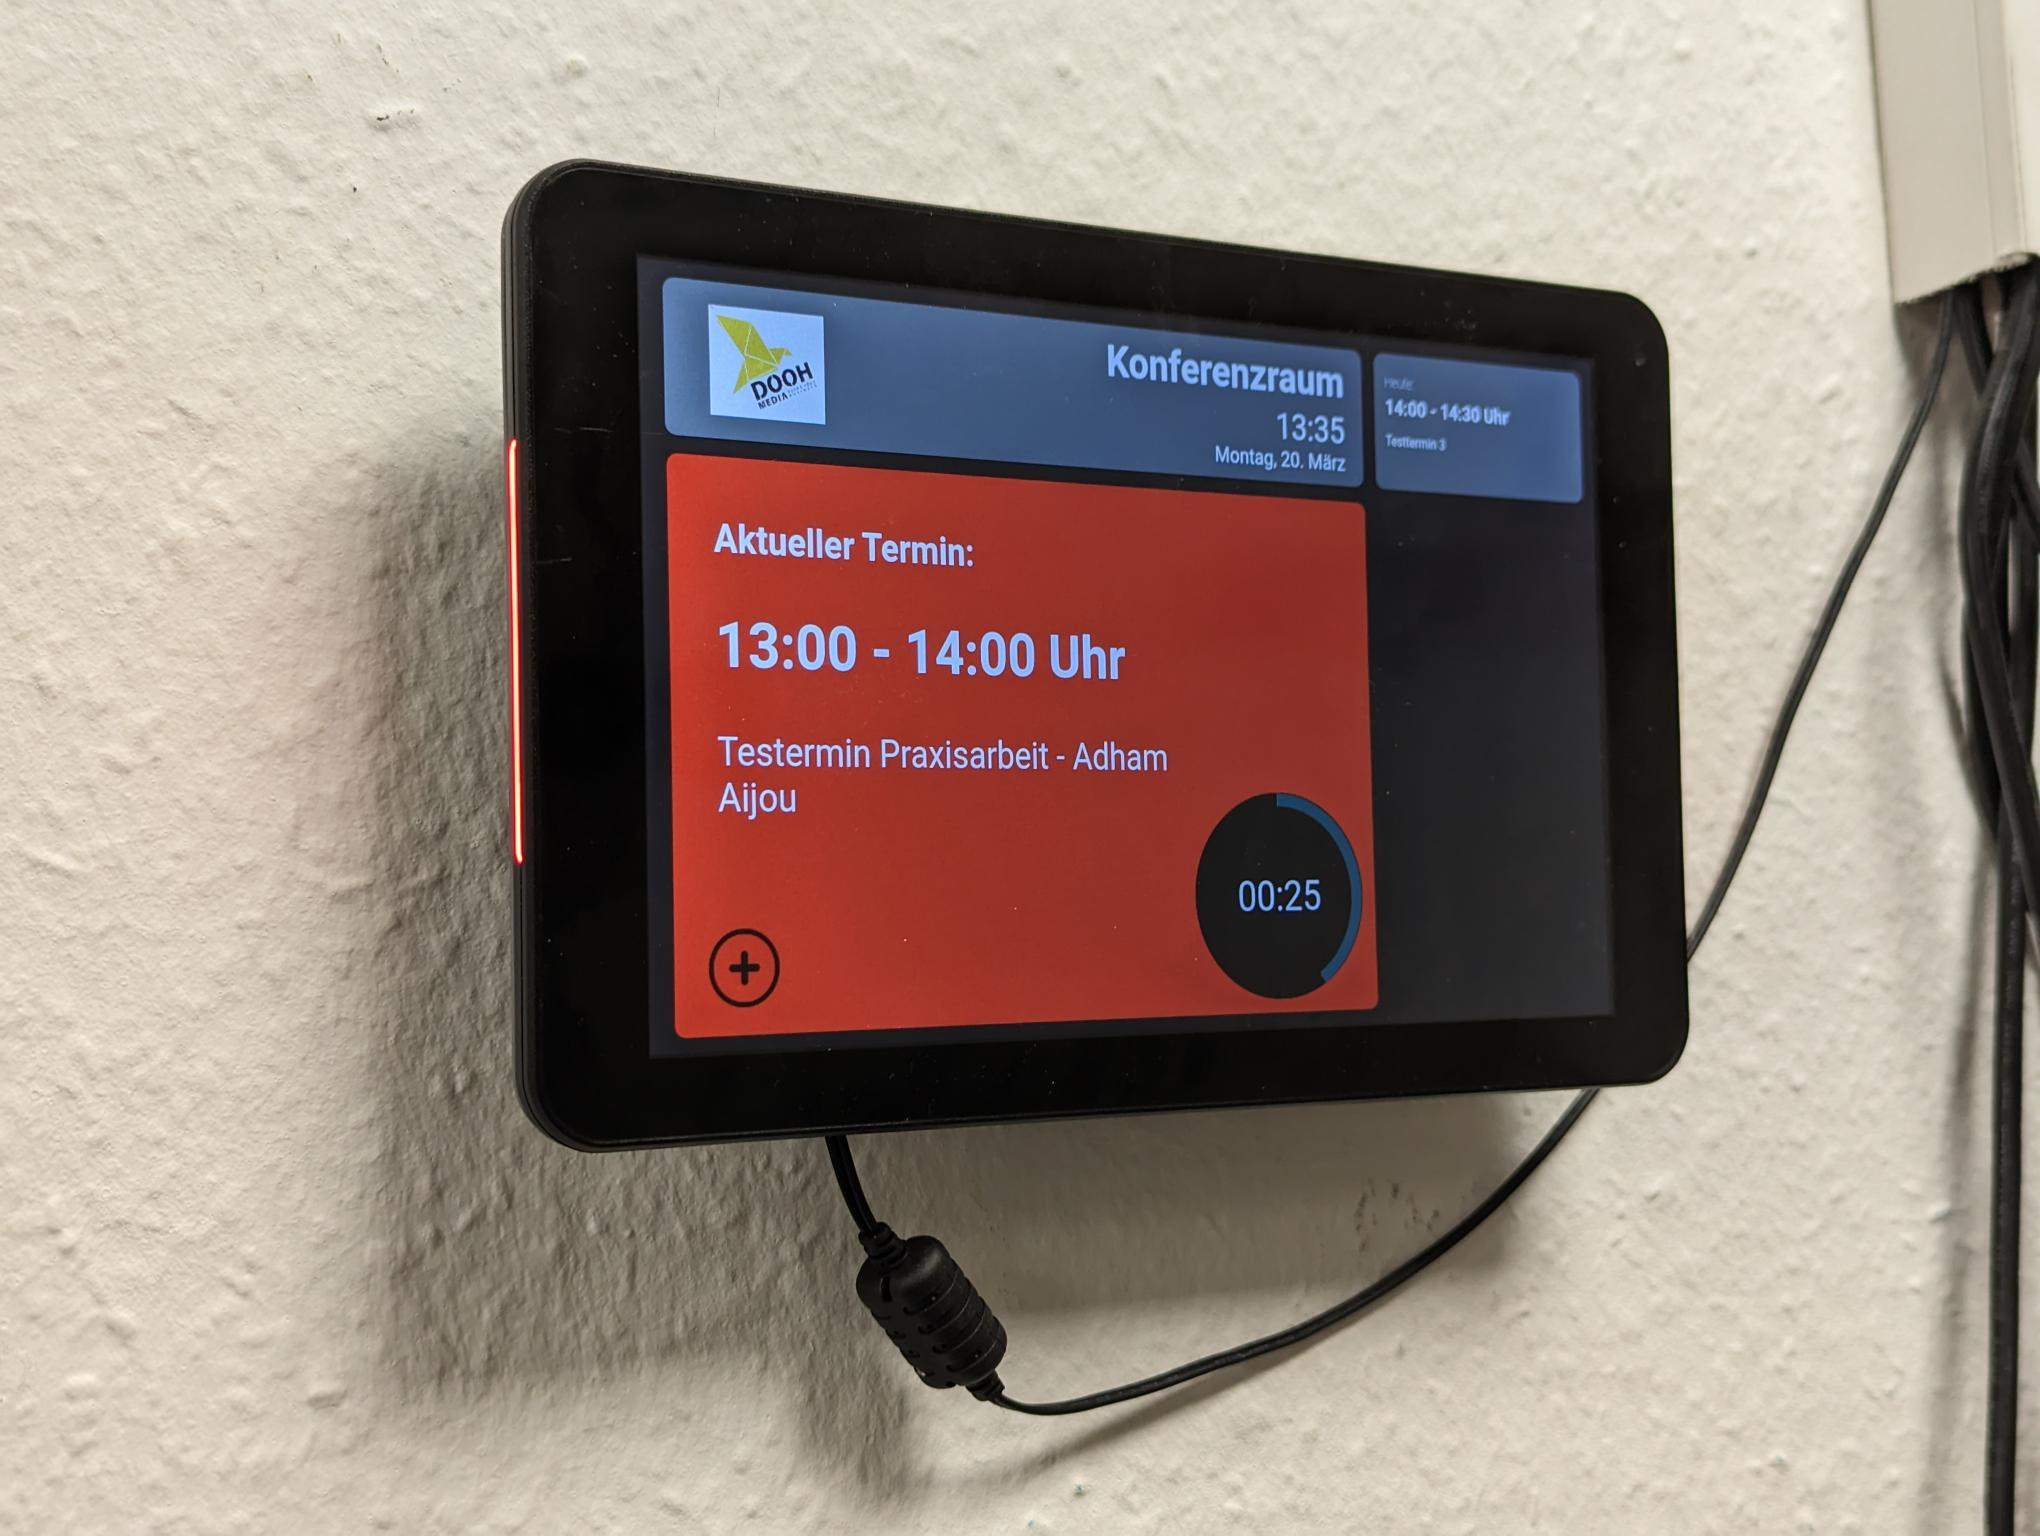
\includegraphics[width=0.5\textwidth]{Bilder/FertigesProdukt}
%    \caption{Fertiges Produkt - Gerät mit der Anwendung}
%    \label{fig:fertiges-produkt}
%\newline
%\newline
%    \end{figure}
\justifying
\newpage
\section{Literaturverzeichnis}\label{sec:literaturverzeichnis}